\clearpage
\subsection{Getting started with MOSL}
\texHeader
\hypertarget{static:starting tex}{}

\hypertarget{static tex}{} 

{\footnotesize If you completed the demo in Part I, your Eclipse workspace will look slightly different than ours depicted in the screenshots. In an effort to
keep things as clear as possible, we have removed the files from our package explorer, but still recommend keeping them for future reference.}

\begin{itemize}
\item[$\blacktriangleright$] Begin a new metamodel project from eclipse by navigating to the \texttt{New Metamodel} button on the toolbar. In the dialog that
appears, enter `LeitnersLearningBox' as the project name, and select \texttt{Textual (MOSL)}  (Fig.~\ref{fig:new_project}).

\vspace{0.5cm}

\begin{figure}[htbp]
	\centering
  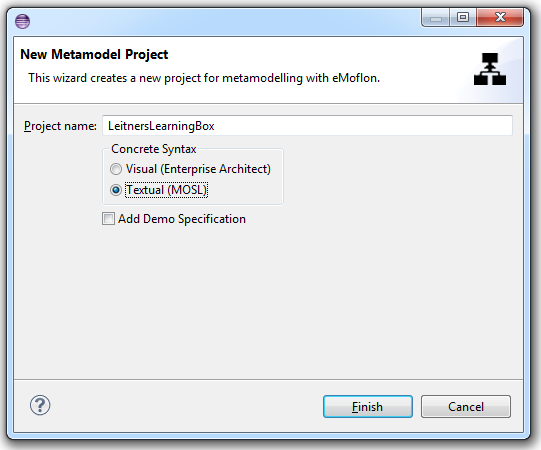
\includegraphics[width=0.8\textwidth]{eclipse_texNewMetamodelPlain}
	\caption{Creating a new metamodel project}
	\label{fig:new_project}
\end{figure}

\vspace{0.5cm}

\item[$\blacktriangleright$] You'll see your new project appear under the ``Specifications" node\footnote{If no nodes are appearing in your package explorer,
make sure your ``Top Level Elements'' are set to ``WorkingSets.''}. If you're interested in the details on eMoflon's project structure, review Section 4.2 from
Part I\footnote{\downLink}. Otherwise, expand the project as deep as it goes (Fig.~\ref{fig:expanded_folders}).

\clearpage

\begin{figure}[htbp]
	\centering
  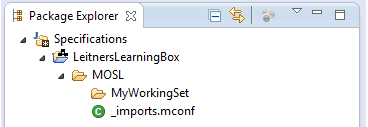
\includegraphics[width=0.6\textwidth]{eclipse_texFoldersExpanded}
	\caption{Expanded project files}
	\label{fig:expanded_folders}
\end{figure} 

\vspace{0.25cm}

\item[$\blacktriangleright$] We're most interested in \texttt{MyWorkingSet}, which represents the project scope. It includes all the technical details required
for code generations, such as those found in the \texttt{\_imports.mconf} file. Right click this folder, and create a new \texttt{EPackage}, naming it
`LearningBoxLanguage'. This is now the container for all your modelling files. In essence, this is the location all your generated files will be derived from.

\item[$\blacktriangleright$] Your package explorer should now resemble Fig.~\ref{fig:preBuild}.

\item[$\blacktriangleright$] To finish initalizing your metamodel, navigate to ``Build (Without cleaning),'' found beside ``New Metamodel'' on the
toolbar (Fig.~\ref{fig:preBuild}).

\vspace{0.25cm}

\begin{figure}[htbp]
	\centering
  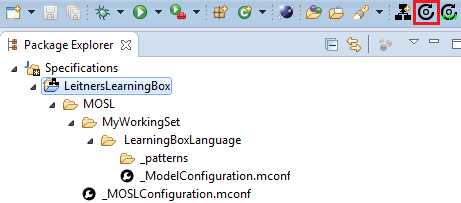
\includegraphics[width=0.8\textwidth]{eclipse_texBuildButton}
	\caption{Inital structure of Leitner's Learning Box}
	\label{fig:preBuild}
\end{figure} 

\vspace{0.25cm}

\item[$\blacktriangleright$] A new, ``MyWorkingSet'' node, named after your project container, should have been created (Fig.~\ref{fig:finalFiles}). The
first key folder in this node is ``gen.'' This is the package where any and all Java files, generated from your metamodel will be placed.

\newpage

\begin{figure}[htbp]
	\centering
  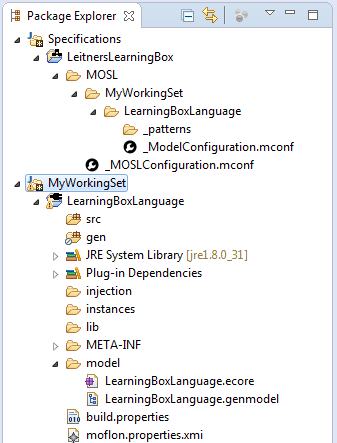
\includegraphics[width=0.5\textwidth]{eclipse_texFinalExpansion}
	\caption{The project fully initialized}
	\label{fig:finalFiles}
\end{figure} 

\vspace{0.5cm}

\item[$\blacktriangleright$] Navigate to ``LearningBoxLanguage/model.'' This folder contains \\ \texttt{LearningBoxLanguage.ecore}, the concrete model of
your metamodel. This will adhere to any types and constraints you define within ``LeitnersLearningBox/MOSL/MyWorkingSet/LearningBoxLanguage.'' Like ``gen,"
its currently empty as we haven't declared any classes (types) or references. This folder also contains a \texttt{.genmodel} file, which contains the technical
details needed for generation, such as build paths.

\vspace{0.5cm}

\item[$\blacktriangleright$] In the next section, we'll start creating the abstract syntax for Leitner's Box, and you'll quickly see each of these elements
grow.

\fancyfoot[R]{$\triangleright$ \hyperlink{static:classes tex}{Next}}

\end{itemize}
